%!TEX root = ../../Master.tex
\section{Implementing Graph Theory}

Navigate from a to b using graph theory is one thing, but implementing graph theory in a C program is a an entirely different thing. This section will cover two methods to represent a graph in computer memory. 

\begin{itemize}
	\item Sequential representation.
	\item Linked list representation.
\end{itemize} 


\subsection{Linked List Representation}
A linked list is defined as "a list implemented by each item having a link to the next item."\cite{linked_list_def}
This means that every item in the list has a element pointing to the next item in the list. This way of structuring the data makes it possible to dynamic manipulate the list.\cite{Linked_List}

Inserting new items to a linked list is relatively easy, compared to a sequentially representation of graph. 
This can be done by redirecting a pointer to a element $A$ in the list to a newly created element $B$, and make the the new element point at location where the first element was pointing to $C$. This example is shown at \cref{fig:link}.

\begin{figure}[h]
 \centering
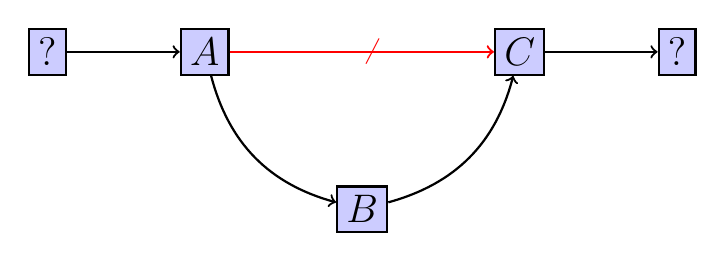
\begin{tikzpicture}[thick,main node/.style={fill=blue!20,draw,font=\sffamily\Large\bfseries}]
  \node[main node] (a) at (0,0) {\(A\)};
  \node[main node] (c) at (4,0) {\(C\)};
  \node[main node] (b) at (2,-2) {\(B\)};
  \node[main node] (d) at (-2,0) {$?$};
  \node[main node] (e) at (6,0) {$?$};
   
   \path[->]
     (d) edge node {$ $} (a)
     (c) edge node {$ $} (e)
     (a) edge [bend right] node {$ $} (b)
     (b) edge [bend right] node {$ $} (c);

  \draw[red,->] (a) to node {\(\not\)} (c);
\end{tikzpicture}
\caption{Linked list example} \label{fig:link}
\end{figure}

\subsection{Sequentially Representation}
A Sequential representation means that the data describing the vertices is placed sequential sequentially in the memory, one vertex after another vertex. 

This requires less memory than using a linked list, because it is known where all the vertices is located relative to each other, in the memory. And this does not apply to a linked list, because all elements in the linked list need to store information about where the next element is located.

Adding new elements to the list is relatively easy compared to sequentially stored data.
It can be done by changing where what the last element of the list is point at, to a new element.
Removing an item can be done similarly by changing the element pointing to the item that is wanted to be removed, so the list skips a element. This is shown in \cref{fig:examplegraph}. %indsæt 

\sinote{fix ny figur}

% \subsection{data structure}
% In this section it will be covered how a graph actual can be represented in the memory, using the above methods. To explain this there examples in the following sections will be based on the graph shown at \cref{fig:graph}.
% \begin{figure}[h]
% \centering
% \begin{tikzpicture}[->,>=stealth',shorten >=1pt,auto,node distance=3cm,
%   thick,main node/.style={circle,fill=blue!20,draw,font=\sffamily\Large\bfseries}]

%   \node[main node] (1) {1};
%   \node[main node] (2) [below left of=1] {2};
%   \node[main node] (3) [below right of=1] {3};
%   \path[-]
%   	(1) edge node {2.0} (3)
%     (2) edge node {1.0} (1)
%     (3) edge node {3.0} (2);
% \end{tikzpicture}
% \caption{example graph} \label{fig:graph}
% \end{figure}




\begin{figure}[h]
\centering
\begin{tikzpicture}[->,>=stealth',shorten >=1pt,auto,node distance=3cm,thick,main node/.style={fill=blue!20,draw,font=\sffamily\Large\bfseries}]

  \tikzset{mystyle/.style={->,relative=false,in=0,out=0,bend left=100,looseness=3}}

  \node[main node] at (0,-2) (2) {$V_1$};
  \node[main node] at (2,-2) (3) {$V_2$};
  \node[main node] at (4,-2) (4) {$V_3$};
  \node[main node] at (0,-4) (5) {$EP_1$};
  \node[main node] at (2,-4) (7) {$EP_2$};
  \node[main node] at (4,-4) (9) {$EP_1$};
  \node[main node,label=below:$1$] at (0,-6) (6) {$E_1$};
  \node[main node,label=below:$1$] at (2,-6) (8) {$E_1$};

   \path[->]
   	(2) edge node {VP} (3)
   	(3) edge node {VP} (4)
   	(2) edge node {EP} (5)
   	(5) edge node {EP} (6)
   	(5) edge node {EP} (7)
   	(7) edge node {EP} (8)
   	(6) edge [bend left=60] node { } (2)
   	(6) edge [bend left=100,looseness=2.3] node { }(3)
   	(8) edge [bend left=100,looseness=2.5] node { }(2)
   	(8) edge [bend right=100,label=right] node { }(4);


\end{tikzpicture}
\caption{example graph} \label{fig:examplegraph}
\end{figure}



\subsection{Representing a Graph as XML}

In order to search through a graph in a C program, the graph needs to be read by the C program. XML was chosen as the markup language for representing a graph, because of it is easy to read for both humans and computers. An example of how a graph is represented as XML is seen in \cref{list:xml_demo}.

\lstinputlisting[language=XML, label=list:xml_demo, caption={An example of a graph represented as XML}]{Chapters/problem_solution/demo_xml.xml}